\documentclass[a4, 14pts]{seminar}
\usepackage[dvips]{pstcol}
\usepackage{semcolor}
\usepackage{sem-page}
\usepackage{slidesec}
\input{seminar.bug}
\input{seminar.bg2}
\usepackage{semhelv}
\usepackage{subfigure}
\usepackage[latin1]{inputenc}
\usepackage[T1]{fontenc}
\usepackage{times}
\usepackage{longtable,array,enumerate}


\usepackage{multicol}

\usepackage[intlimits,sumlimits,namelimits]{amsmath}
\usepackage{amssymb}
\usepackage[mathscr]{eucal}
\usepackage{mathrsfs}
\usepackage{amsthm}
\usepackage{amsfonts}
\usepackage{amsmath}

\usepackage[dvips]{graphicx}
\usepackage{epsf}
\usepackage{epsfig}
\usepackage{fancyhdr}
\usepackage{layout}

\usepackage[french]{babel}
\usepackage[T1]{fontenc}
\usepackage[latin1]{inputenc}

\usepackage{url}
\usepackage{xspace}

\newtheorem{corollary}{Corollaire}[section]
\newtheorem{definition}[corollary]{D\'{e}finition}
\newtheorem{equations}[corollary]{Equations}
\newtheorem{example}[corollary]{Exemple}
\newtheorem{lemma}[corollary]{Lemme}
\newtheorem{proposition}[corollary]{Proposition}
\newtheorem{remark}[corollary]{Remarque}
\newtheorem{theorem}[corollary]{Th\'{e}or\`{e}me}
	    %%% The above 7 commands are used in the following way:
	    %%% The definition environment, for example, is created by
	    %%% \begin{definition}\label{xxx}. . .\end{definition}
\newcommand{\mylabel}[1]{\label{#1}
			\ifx\undefined\stillediting
			\else \fbox{$#1$}\fi }
\newcommand{\BE}{\begin{equation}}
\newcommand{\BEQ}[1]{\BE\mylabel{#1}}
\newcommand{\EEQ}{\end{equation}}
\newcommand{\rfb}[1]{\mbox{\rm
	      (\ref{#1})}\ifx\undefined\stillediting\else:\fbox{$#1$}\fi}
\newcommand{\half}   {{\frac{1}{2}}}
\newenvironment{matr}[1]{\left[ \begin{array}{#1}}{\end{array}	\right]}

\newfont{\Blackboard}{msbm10 scaled 1200}
\newcommand{\bl}[1]{\mbox{\Blackboard #1}}
\newfont{\roma}{cmr10 scaled 1200}

\newcommand{\propp}{{\hskip -2.2mm{\bf .}\hskip 3mm}}

\newcommand{\ovra}{\overrightarrow}
	    % fin des commandes de Marius

\fancyhf{}
\renewcommand\headrulewidth{0.2mm}
\renewcommand\footrulewidth{0.2mm}


\newcommand{\R}{\mathbb{R}}
\newcommand{\C}{\mathbb{C}}
\newcommand{\N}{\mathbb{N}}
\newcommand{\Z}{\mathbb{Z}}

\newcommand{\ROT}{{\text{Rot}}}
\newcommand{\Rot}{\vec{\text{Rot}}}
\newcommand{\rot}{\vec{\text{rot}}}

\newcommand{\dsp}{\displaystyle}

\usepackage{mathtools}
\DeclareMathOperator{\Mat}{Mat}
\DeclarePairedDelimiter{\diagfences}{(}{)}
\newcommand{\diag}{\operatorname{diag}\diagfences}
\newcommand\bigzero{\makebox(0,0){\text{\huge0}}}
\newcommand{\E}{\mathrm{E}}
\newcommand{\Var}{\mathrm{Var}}
\newcommand{\Cov}{\mathrm{Cov}}

\newcommand\eads{\textsf{}\xspace}
\newcommand\eadsccr{\textsf{}\xspace}

\fancyhead[L]{\theslideheading}
\fancyhead[R]{\textcolor{blue}{\eadsccr \thepage }}
\fancyfoot[R]{\textcolor{blue}{}}
\fancyfoot[L]{\textcolor{blue}{}} %% today
\renewcommand\headwidth{\textwidth}
\autoslidemarginstrue

\newslideframe{%
	      myscshadow}[\SemcolorFrameOps
	      \psset{shadowcolor=green}]{\psshadowbox{#1}}
\newcommand{\ud}{\mathrm{d}}

\newcommand{\ds}{\displaystyle}
\slideframe{myscshadow}
\setlength\slideframewidth{.5pt}
\setlength\footskip{1cm}
\setlength\headsep{1cm}

	    %\renewcommand\makeslideheading[1]{\par
	    %   \framebox{\theslidesection. #1}\par
	    %}
	    %\renewcommand\makeslidesubheading[1]{\par
	    %   \leavevmode\hspace*{1cm}%
	    %   \alph{slidesubsection}. #1\par
	    %}

\definecolor{Pink}{rgb}{1.,0.,0.2}
\definecolor{Mygreen}{rgb}{0.3,0.7,0.6}

\renewcommand\makeslideheading[1]{\par
	      \fcolorbox{black}{Mygreen}{\color{yellow}\theslidesection. #1}\par
	    }
\renewcommand\makeslidesubheading[1]{\par
	      \leavevmode\hspace*{1cm}%
	      \textcolor{Mygreen}{\alph{slidesubsection}. #1}\par
	    }

\makeatletter
\renewcommand\slide@contents{\par
	      \begin{center}
	\Large \bfseries\textcolor{blue}{Plan}
	      \end{center}
	      \def\l@slide##1##2##3{%
		\@undottedtocline{1}{1.5em}{2.3em}{\slidenumberline{##1.}{##2}}{}}%
	      \def\l@subslide##1##2##3{%
		\@undottedtocline{1}{1.5em}{3.3em}{\slidenumberline{\@alph{##1})}{##2}}{}}%
	      \@startlos
	    }
\makeatother

\slideframe{none}
	    %\XgrDefinitFormat{*}{line=0,mark=0,ll=1}
	    %\XgrDefinitFormat{pr}{}
	    %\XgrDefinitFormat{ks}{line=-1,mark=8,ll=0.4}
\begin{document}
\slidepagestyle{fancy}
	    %%%%%%%%%%%%%%%%%%%%%%%%%%%%%%%%%%%%%%%%%%%%%%%%%%%%%%%%%%%%%%%%%%%%%%%%%%%
\begin{slide}
\thispagestyle{plain}
\begin{center}
\textcolor{blue}{\huge  Multi risk factor model}\\
\textcolor{blue}{\huge  Constraint Variance optimization}\\
\textcolor{blue}{\huge  Long/short 100/100 market portfolio}\\
\textcolor{blue}{\huge  Long/short 130/30 portfolio}\\
\vspace{0.25 cm}
\textbf{DUPREY Stefan}\\
\small{\textbf{}\\ 

	    }
	    %\eadsccr
\end{center}
\end{slide}
	    %%%%%%%%%%%%%%%%%%%%%%%%%%%%%%%%%%%%%%%%%%%%%%%%%%%%%%%%%%%%%%%%%%%%%%%%%%
	    %%%%%%%%%%%%%%%%%%%%%%%%%%%%%%%%%%%%%%%%%%%%%%%%%%%%%%%%%%%%%%%%%%%%%%%%%%%
	    {\small{
\begin{slide}
\slidecontents
\renewcommand\theslideheading{Plan}
\end{slide}

%%%%%%%%%%%%%%%%%%%%%%%%%%%%%%%%%%%%%%%%%%%%%%%%%%%%%%%%%%%%%%%%%%%%%%%%%%%
%%%%%%%%%%%%%%%%%%%%%%%%%%%%%%%%%%%%%%%%%%%%%%%%%%%%%%%%%%%%%%%%%%%%%%%%%%%
{\small{
\begin{slide}
\slideheading{Factor model and stochastic processes}
We have $N\in\mathbb{N}$ stocks. Their returns $R_i, \forall i \in \{1,\cdots,N\}$ are modeled by $N$ random processes  $\chi_i$
corresponding to idiosyncratic risk together with $K$ random processes $f_A$ :
\begin{equation}
R_i = \chi_i + \sum_{A=1}^{K}\widetilde{\Omega}_{iA}f_A
\end{equation}
\begin{equation}
\langle \chi_i, \chi_j \rangle = \xi_{ij}^2 \delta_{ij}
\end{equation}
\begin{equation}
\langle \chi_i, f_A \rangle = 0
\end{equation}
\begin{equation}
\langle f_A,f_B \rangle = \Phi_{AB}
\end{equation}
\begin{equation}
\langle R_i,R_j \rangle = \Theta_{ij}
\end{equation}
\end{slide}
\begin{slide}
\slideheading{Covariance matrix}
The $R_i$ covariance matrix can be written as :
\begin{equation}
\Theta = \Xi + \widetilde{\Omega}\Phi\widetilde{\Omega}^{\intercal}
\end{equation}
where $\Xi_{ij}=\xi_{ij}^2 \delta_{ij}$ is the diagonal idiosyncratic part of the variance and $\Phi$ the $K\times K$ factor covariance matrix, $\widetilde{\Omega}$ is the $K\times K$ factor
loading matrix.
\newline
Note that $K < < N$ gives more out of samples stability. Through Cholesky :
\begin{equation}
\Theta = \Xi + \Omega\Omega^\intercal
\end{equation}
where $\Omega = \widetilde{\Omega}\widetilde{\Phi}$ and $\widetilde{\Phi}\widetilde{\Phi}^\intercal=\Phi$
\newline
Note that the standard variance for a portfolio with weights $\omega$ decomposes as :
\begin{equation}
\omega^\intercal \Omega \omega =  \sum_{i=1}^{N}  \xi_{ij}^2 + f^\intercal \Phi f
\end{equation}
where $f = \Omega \omega$ is the factor values for our portfolio with weights $\omega$
\end{slide}
\begin{slide}
\slideheading{Regressing returns over factor loading/exposure}
At each observation time we have to regress our stock returns to our stock factors :
\begin{equation}
R(t) = \sum_{k=1}^{K} \beta_k(t) \times F_k(t) + \epsilon(t)
\end{equation}
\begin{equation}
R(t) = \sum_{k=1}^{K} f_k(t) \times \Omega_k(t) + \epsilon(t)
\end{equation}
$\Omega_i$, $F_i$ is the factor exposure or loading for the stock $i$ and $\beta_i$, $f_i$ is the factor return or factor itself.
\newline
The variance of $\epsilon(t)$ is the idiosyncratic risk for stock $i$
\newline
The covariance of $(f_k(t))_{k \in \{1,\cdots,K\}}$ is the factor covariance matrix.
\newline
Here a proprietary strategy is to be defined to compute the factor matrix : a rolling standard deviation or garch volatility estimation for idiosyncratic variance and a rolling Ledoit-Wolf covariance matrix estimation
\end{slide}
{\small
\begin{slide}
\slideheading{Minimum variance optimization rebalancement at each date}
\begin{equation}
\displaystyle
\operatornamewithlimits{argmin}_{\begin{cases}
\omega \in \mathbb{R}^N,\omega_i > 0,\omega_i < 1\\
\sum_{i=1}^{N}\omega_i = 1\\
\newline \sum_{i=1}^{n} \omega_i \beta_i =\sum_{i=1}^{n} \omega_i \frac{\Cov \left(R_i,R_{market} \right)}{\Var (R_i)} = 1
\end{cases}
} \left\{  \omega \Sigma \omega^\intercal - q\times \mu^\intercal\omega\right\}, \ becomes 
\end{equation}
\begin{equation}
\displaystyle
\operatornamewithlimits{argmin}_{\begin{cases}
x=(f,\omega) \in \mathbb{R}^{(N+K)},\omega_i > 0,\omega_i < 1\\
\sum_{i=1}^{N}\omega_i = 1\\
\sum_{i=1}^{n} \omega_i \beta_i =\sum_{i=1}^{n} \omega_i \frac{\Cov \left(R_i,R_{market} \right)}{\Var (R_i)} = 1 \\
\Omega \omega = f
\end{cases}
}\left\{  x Q x^\intercal - q\times \widetilde{\mu}^\intercal x\right\}
\end{equation}
where :
\begin{equation}
\displaystyle
Q=\left(
\begin{array}{c|c}
  \Phi & 0 \cdots 0 \\ \hline
  0 & \begin{array}{cccc}
\xi_{11}^2&& \ \ \bigzero \\
&\ddots\\
&&\ddots\\
\bigzero \ &&& \xi_{nn}^2
\end{array} \\[-4ex]
  \vdots & \\[-0.5ex]
  0 &
\end{array}
\right),\displaystyle
\widetilde{\mu}=\left(
\begin{array}{c}
  0  \\
  \mu 
\end{array}
\right)
\end{equation}
\end{slide}
}
\begin{slide}
\slideheading{Long/short 130/30 portfolio}
\begin{equation}
\displaystyle
\operatornamewithlimits{argmin}_{\begin{cases}
x=(f,\omega) \in \mathbb{R}^{(N+K)}\\
v \in \mathbb{R}^{(N)}\\
-0.1<\omega_i<0.1\\
\sum_{i=1}^{N}\omega_i = 1\\
\sum_{i=1}^{n} \omega_i \beta_i =\sum_{i=1}^{n} \omega_i \frac{\Cov \left(R_i,R_{market} \right)}{\Var (R_i)} = 1 \\
\Omega \omega = f \\
-v<\omega<v \\
v > 0 \\
\sum_{i=1}^{N}v_i = 1.6
\end{cases}
}\left\{  x Q x^\intercal - q\times \widetilde{\mu}^\intercal x\right\}
\end{equation}
where :
\begin{equation}
\displaystyle
Q=\left(
\begin{array}{c|c}
  \Phi & 0 \cdots 0 \\ \hline
  0 & \begin{array}{cccc}
\xi_{11}^2&& \ \ \bigzero \\
&\ddots\\
&&\ddots\\
\bigzero \ &&& \xi_{nn}^2
\end{array} \\[-4ex]
  \vdots & \\[-0.5ex]
  0 &
\end{array}
\right),\displaystyle
\widetilde{\mu}=\left(
\begin{array}{c}
  0  \\
  \mu 
\end{array}
\right)
\end{equation}
\end{slide}
\begin{slide}
\slideheading{Long/Short 100/100 Market Neutral portfolio}
\begin{equation}
\displaystyle
\operatornamewithlimits{argmin}_{\begin{cases}
x=(f,l\omega, s\omega) \in \mathbb{R}^{(N+3*K)}\\
b \in \mathbb{R}^{(N)}\\
0<l\omega_i<0.1, 0<s\omega_i<0.1\\
\sum_{i=1}^{N}l\omega_i = \sum_{i=1}^{N}s\omega_i\\
\sum_{i=1}^{N}l\omega_i + \sum_{i=1}^{N}s\omega_i = 2\\
\sum_{i=1}^{n} l\omega_i \beta_i = \sum_{i=1}^{n} s\omega_i \beta_i \\
\Omega l\omega - \Omega s\omega  = f \\
l\omega < b \\
s\omega < 1-b
\end{cases}
}\left\{  x Q x^\intercal - q\times \widetilde{\mu}^\intercal x\right\}
\end{equation}
where :
\begin{equation}
\displaystyle
Q=\left(
\begin{array}{c|ccc}
  \Phi & 0 \cdots 0 \\ \hline
  0 &  Q_{idio} & -Q_{idio}\\
  0 & -Q_{idio}& Q_{idio}
\end{array}
\right),
\displaystyle
Q_{idio} = \left(\begin{array}{cccc}
\xi_{11}^2 && \ \ \bigzero \\
&\ddots\\
&&\ddots\\
\bigzero \ &&& \xi_{nn}^2
\end{array}
\right)
\end{equation}
\end{slide}

\begin{slide}
\slideheading{R code : computing factors loadings}
\begin{center}
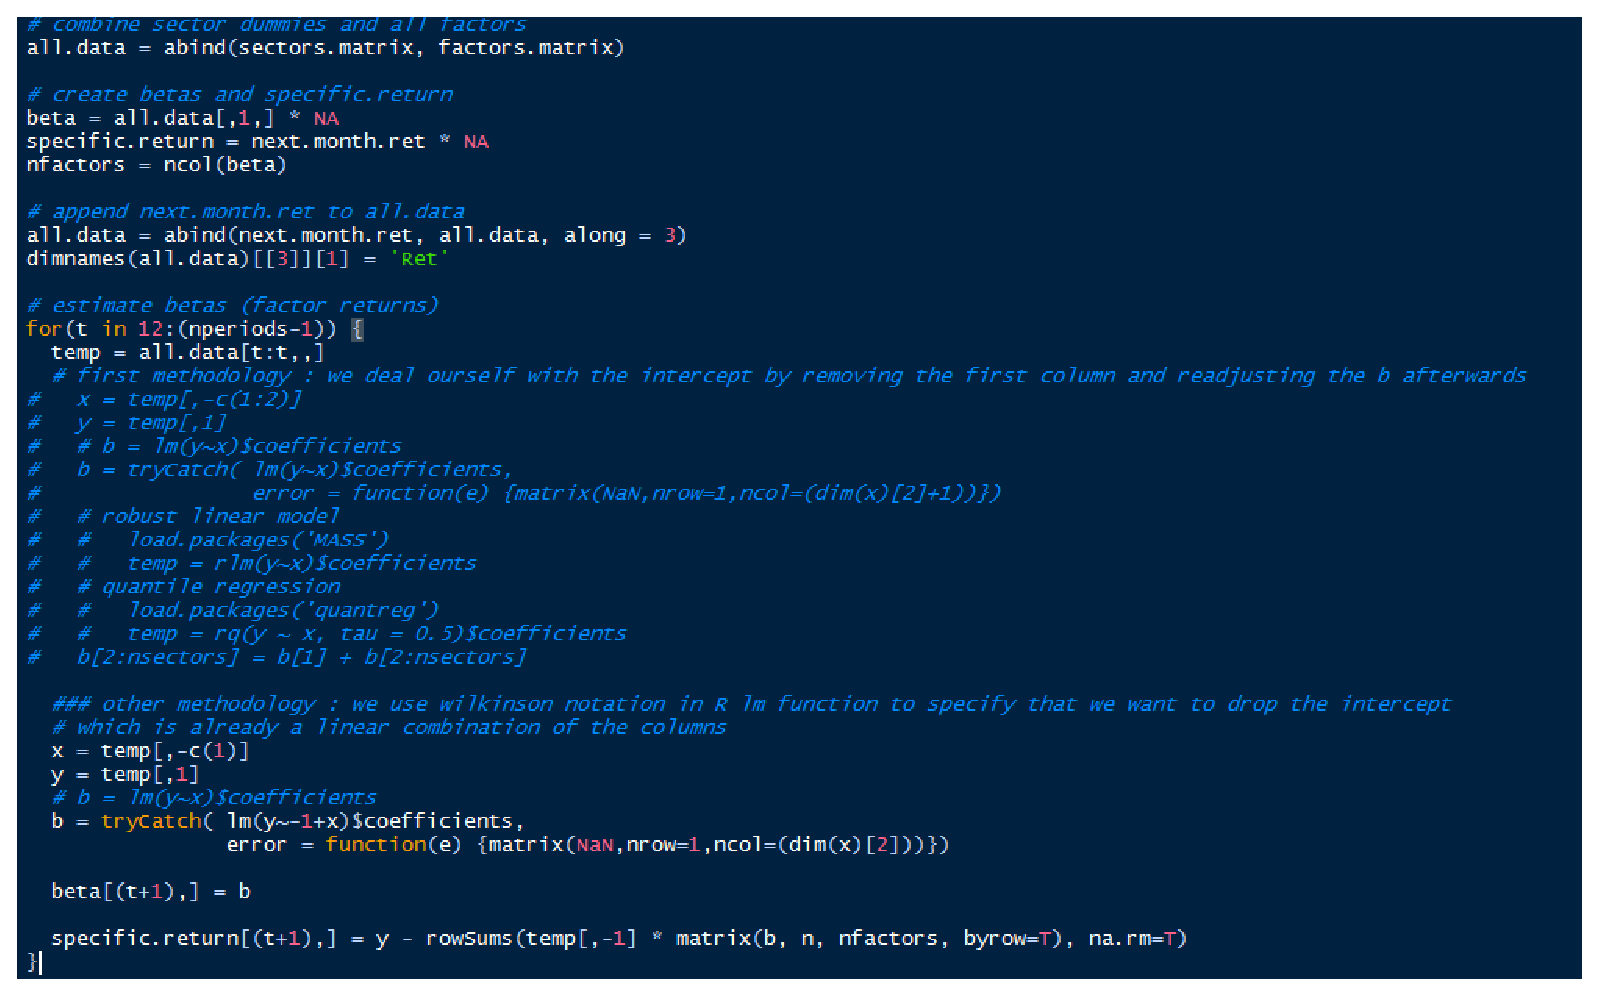
\epsfig{file=computing_factor_loading.eps,height=6.5cm,width=7.5cm}
\end{center}
\end{slide}
\begin{slide}
\slideheading{R code : estimating factors covariance matrix and idiosyncratic risk}
\begin{center}
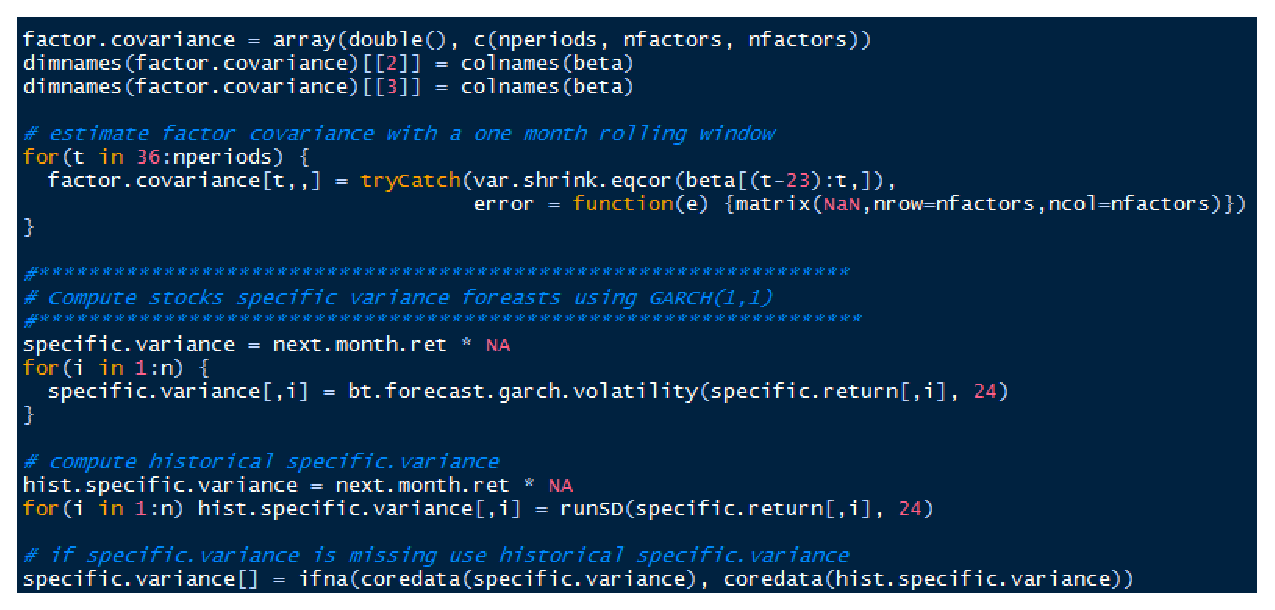
\epsfig{file=computing_factor_covariance_idiosyncratic_risk.eps,height=4.5cm,width=7.5cm}
\end{center}
\end{slide}
\begin{slide}
\slideheading{R code : quadratic programming, constraints and multi risk factor models}
\begin{center}
\epsfig{file=computing_long_short_market_neutral_constraint.eps,height=7cm,width=7.5cm}
\end{center}
\end{slide}
\end{document}
